\documentclass[12pt,a4paper]{article}
\usepackage[utf8]{inputenc}
\usepackage{amsmath}
\usepackage{amsfonts}
\usepackage{amssymb}
\usepackage[pdftex]{graphicx}     
\usepackage[french]{babel}
\usepackage{xcolor}
\title{Monitoring de l'alimentation du Maser}
\author{Ibrahim Khaled}
\date{}
\begin{document}
\maketitle
\section*{Quelques explications:}
On veut réaliser un système qui s'assurent que le Maser du bureau de l'heure est toujours alimenté. Sachant que ce dernier peut être alimenté de deux manières: 

\begin{itemize}
\item[-]Secteur (avec convertisseur AC/DC)
\item[-]Batterie 26V

\end{itemize}

\bigskip

Via ce système, on pourra localiser suivant différents cas de figurent où se trouve la panne d'alimentation et envoyer un mail, sms aux responsables du bureau grâce au réseau local. 

\section*{Montage:}  
Le montage se présente comme suit: 

\begin{figure}[!h]
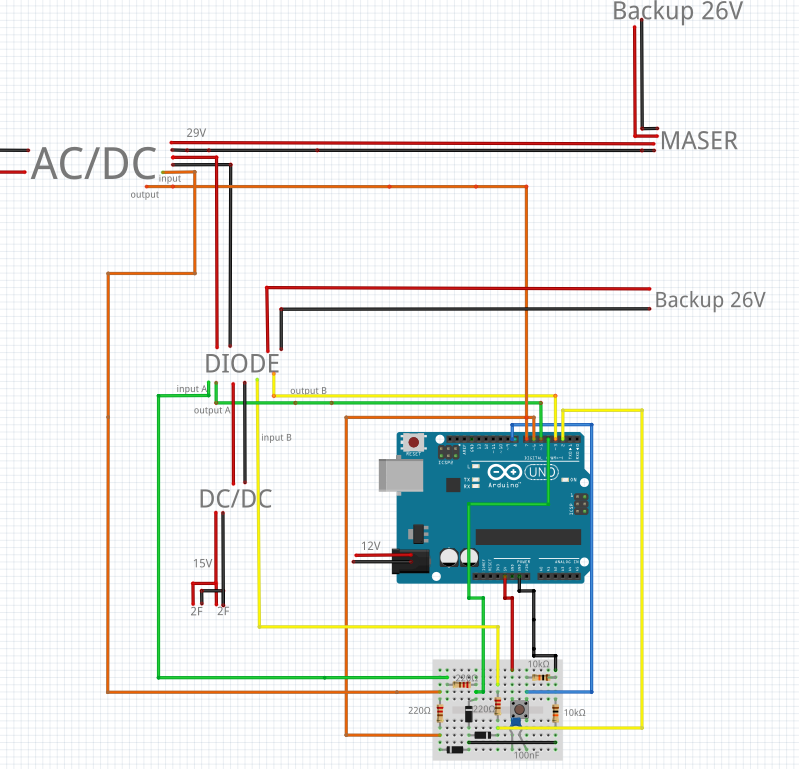
\includegraphics[scale=0.7]{circuit_MASER3.PNG}
\caption{Schéma descriptif}
\end{figure}


\begin{figure}[!h]
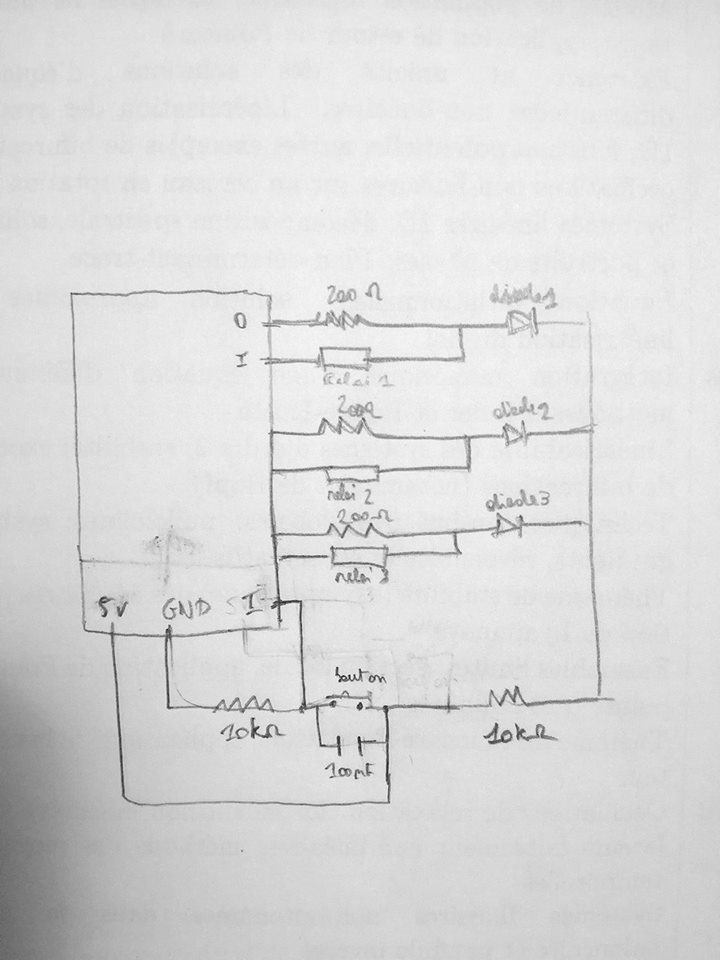
\includegraphics[scale=0.30]{SCHEMA.jpg}
\caption{Schéma en bloque zoom sur la partie connexion avec l'Arduino}
\end{figure}



\newpage
on y retrouve le convertisseur AC/DC pour l'alimentation du Maser, la diode qui joue l'échange de rôle d'alimentation entre le backup batterie et le secteur et enfin un convertisseur DC/DC pour alimenter les doubleurs de fréquences. 

\newpage

Dans ce système, on a 3 relais:
\bigskip

\begin{itemize}
\item[$^{\circ}$] Relai 1: Pour vérifier l'état du convertisseur AC/DC (s'il est fonctionnel)

\bigskip

\item[$^{\circ}$] Relai 2: Control de la sortie A de la diode(permet de vérifier si la diode laisse bien passer le courant venant de l'AC/DC)

\bigskip

\item[$^{\circ}$] Relai 3: Control de la sortie B de la diode(permet de vérifier si la diode laisse bien passer le courant venant de la backup batterie
\end{itemize}

\bigskip
Remarque: Le Maser est continuellement alimenté par les deux sources (cas optimal)
\newpage
\section*{Programme:}
Avant de programmer la logique du système, il faut lister les différents cas de figure qui vont engendrer des erreurs lors d'une panne. 

\begin{figure}[!h]
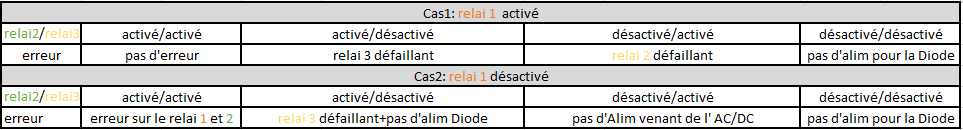
\includegraphics[scale=0.60]{ERREURS.PNG}
\caption{tableau des différentes erreurs possibles}
\end{figure}
\begin{footnotesize}
\begin{flushright}
\begin{itemize}
\item  \textcolor{orange}{Relai 1}
\item  \textcolor{green}{Relai 2}
\item  \textcolor{yellow}{Relai 3}
\end{itemize}
\end{flushright}
\end{footnotesize}

La logique du code est alors la suivante:
\begin{figure}[!h]
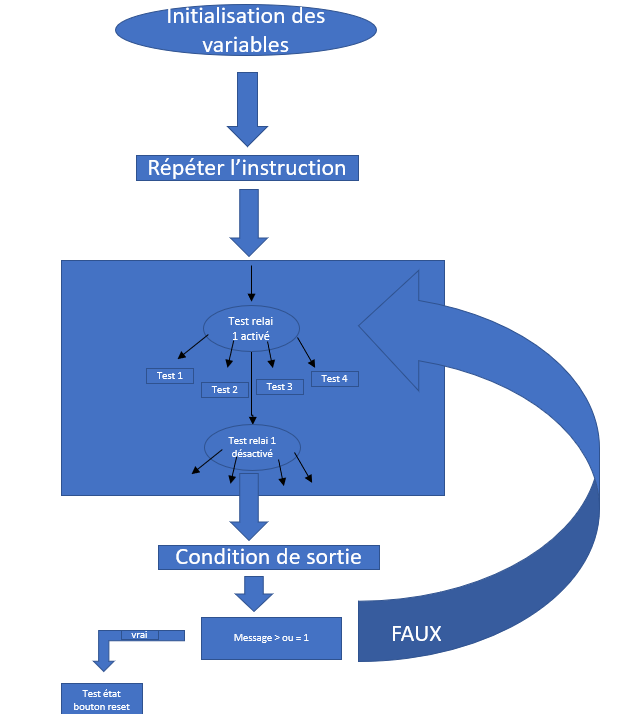
\includegraphics[scale=0.55]{structure.PNG}
\caption{Schéma de la logique du code}
\end{figure}
\newpage
Sachant que pour effectuer un test sur les relai, on envoit un signal avec l'Arduino et on vérifier si l'état du relai est haut (alors il est activé) ou bas (désactivé). Après avoir repéré les erreurs, on envoit le mail et le sms via la fonction préalablement implémenté. On finit le code avec le test du bouton reset qui permet aux responsables de relancer le système lorsque la panne est résolu et d'envoyer une notification qui confirme que le problème est résolu. 

\bigskip

Remarque: Afin d'éviter les spams, on choisit de passer par une variable qui limite l'envoie des messages d'erreurs. On a aussi une variable qui référence les différents types d'erreurs afin d'avoir une précision de l'erreur lors de l'envoie du mail/sms.


\end{document}